\begin{figure*}[t]
\centering
% Vector drawing generated by tools/figures/architecture.py; rerun it after changing the figure.
\ifbilingual
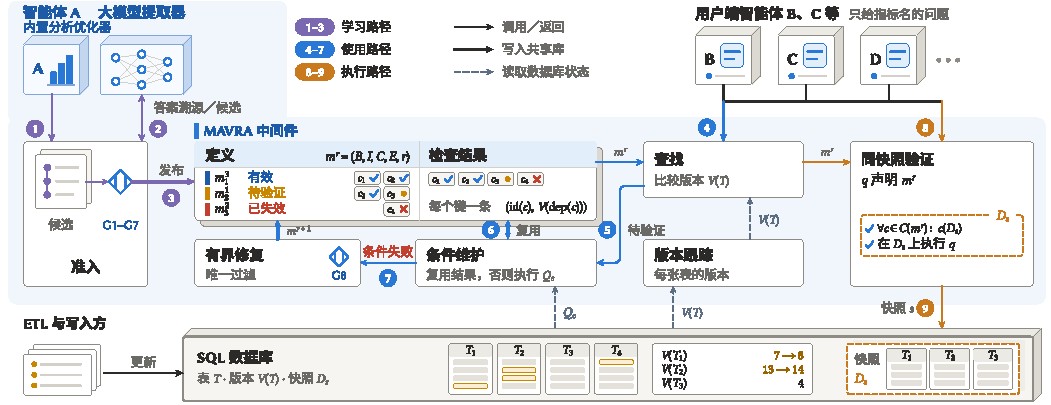
\includegraphics[width=\textwidth]{figures/architecture-zh}
\else
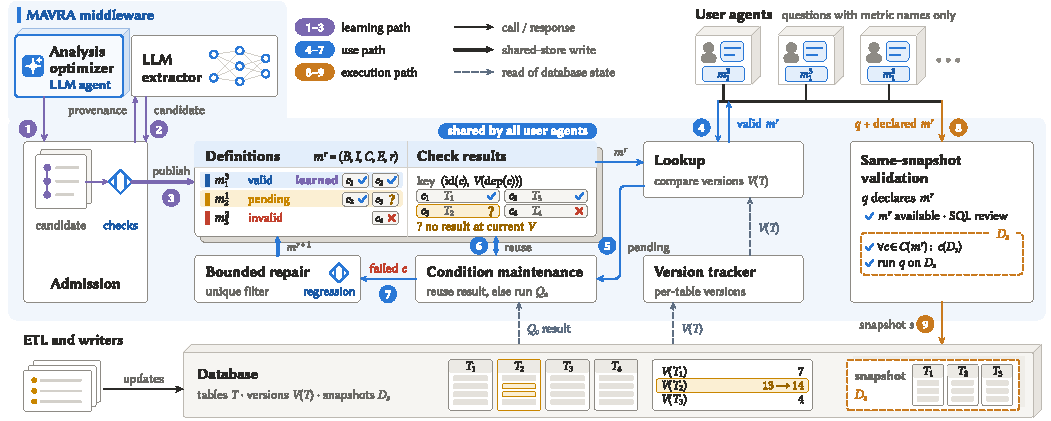
\includegraphics[width=\textwidth]{figures/architecture}
\fi
\caption{\bt{\system\ overview: a user agent's two requests across the three modules. Use path (1--5): a text request names a metric; request handling reads its definition from the shared store, maintenance first revalidates a definition whose tables changed, and only a valid revision is returned. Execution path (6--8): an SQL request declares that revision; same-snapshot validation checks its conditions on the query's snapshot and runs the query there. Learning path: the built-in analysis optimizer, an LLM agent, learns the definitions that admission publishes.}{\system\ 概览：用户端智能体的两种请求在三个模块之间的流转。使用路径（1--5）：文本请求给出指标名；请求处理从共享知识库读取定义，所读表有变化的定义先经维护重验证，只返回有效修订。执行路径（6--8）：SQL 请求声明该修订；同快照验证在查询的快照上核对其条件并在其上执行查询。学习路径：内置分析优化器（大模型智能体）学习定义，经准入后发布。}}
\label{fig:architecture}
\Description{A user agent on the left asks in text for the return amount in May and later sends SQL that declares revision 2 of that definition. Inside the MAVRA middleware sit three modules side by side: request handling with lookup and same-snapshot validation; the shared store with definitions (return amount pending, store revenue valid) and check results kept per table version; and learning and maintenance with the built-in analysis optimizer, an LLM agent, and maintenance, which rechecks, repairs, or invalidates. Blue steps 1 to 5 run from the agent to lookup, from the store to lookup, from the pending definition to maintenance, from maintenance back into the store, and from lookup back to the agent with a valid definition. Orange steps 6 to 8 run from the agent's SQL query to same-snapshot validation, between validation and the check results, and back to the agent with the query result. A thick violet arrow publishes learned definitions into the store. Below, a SQL database holds the query's snapshot, the table versions, in which store\_returns moved from 14 to 15, and the tables; ETL writers update it, validation runs the query on the snapshot, maintenance runs check queries, and the store reads table versions.}
\end{figure*}
